\chapter{Calico}

% [anticpated/actual features]
% [purpose, how does it work]
% [supports designers in sketching]

\section{Canvas and Grid}

\begin{figure}[htb]
\centering
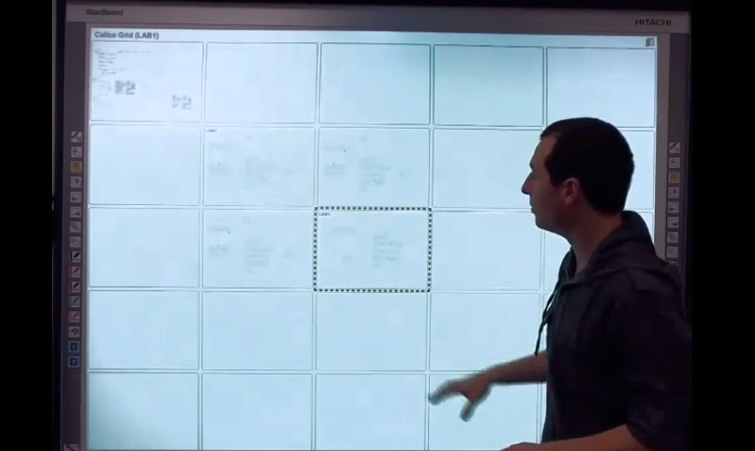
\includegraphics[width=0.8\textwidth]{grid.jpg}
\caption{The grid view within Calico}
\label{fig:grid}
\end{figure}
The grid is the focal point of any session in Calico. It shows the various canvases that users may interact with in a given session. Users may perform various operations on canvases from the grid, such as duplicating or clearing individual cells. The grid also gives a clear overview of the designs that are happening in a session.

\section{Gestures}

\section{Scraps}
Scraps in Calico can be thought of as ``scraps of paper'' that one would place on a desk or on a white board.
Scraps can be easily relocated to different parts of the screen, or even other canvases.
Scraps can be stacked on top of each other and then treated as a unit or group.
By treating scraps as if they were pieces of paper, we [make it easy to understand the manipulation], as designers can easily relate Calico to their current design 

\section{Palette}
The palette in Calico provides users with a ``drawer'' that can easily be used to store commonly used shapes and artifacts. The palette can be synchronized across sessions so that other users in the session can share the same palette.